
%Figure ~\ref{} - \ref{} show the result of our SteinGAN. 
\section{Empirical Results}  \label{sec:gan}

We evaluated our SteinGAN on four datasets,  
MNIST, CIFAR-10, CelebA \citep{liu2015faceattributes}, and Large-scale Scene Understanding (LSUN) \citep{yu2015lsun}, on which we find our method tends to generate realistic-looking images competitive with, sometimes better than DCGAN \citep{radford2015unsupervised} (see Figure~\ref{fig:cifar10} - Figure~\ref{fig:face}). 
% mnist \footnote{\url{http://yann.lecun.com/exdb/mnist/}}
% cifar10 \footnote{\url{https://www.cs.toronto.edu/~kriz/cifar.html}}
% celeba  \footnote{\url{http://mmlab.ie.cuhk.edu.hk/projects/CelebA.html}}
% lsun \footnote{\url{http://lsun.cs.princeton.edu/2016/}}
%In particular, we find we generate better images than DCGAN on CelebA (Figure~\ref{fig:face}), and our simulated CIFAR-10 images achives better testing classification accuracy when used as a training data (see Figure~\ref{fig:cifar10}). 
%generative adversarial networks. 
%See Appendix~\ref{sec:gan} for more information. 
%We will provide code to reproduce our experiments. 
Our code is available at \url{https://github.com/DartML/SteinGAN}.

%\subsection{Implementation}
\newcommand{\enc}{\mathrm{E}}
\newcommand{\dec}{\mathrm{D}}
\paragraph{Model Setup} In order to generate realistic-looking images, we define our energy model based on an autoencoder: 
\begin{align}\label{equ:px}
%p(x|\theta) \propto \exp(-\phi(x,\theta)),~~~~~ \text{where~~~~}  \phi(x, \theta) = \alpha || x -   dec(enc(x))  |, 
p(x|\theta) \propto \exp(-  || x -   \dec(\enc(x;~ \theta);~\theta) ||), 
\end{align}
where $x$ denotes the image. 
This choice is motivated by Energy-based GAN \citep{zhao2016energy} in which the autoencoder loss is used as a discriminator but without a probabilistic interpretation. 
We assume $f(\eta;~\xi)$ to be a neural network whose input $\xi$ is a $\dilincheck{100}$-dimensional random vector drawn by $\mathrm{Uniform}([-1,1])$. 
The positive definite kernel in SVGD is defined by the RBF kernel on the hidden representation obtained by the autoencoder in \eqref{equ:px}, that is, 
$$
k(x, x') = \exp(-\frac{1}{h^2} ||\enc(x;~\theta) - \enc(x';~\theta)||^2). 
$$
As it is discussed in Section~\ref{sec:amortizedsvgd}, the kernel provides a repulsive force 
to produce an amount of variability required for generating samples from $p(x)$. 
%to encourage diversity on the generated samples. % via the term $\nabla_x k(x,x')$ in \eqref{equ:update11}. 
This is similar to the heuristic repelling regularizer in \citet{zhao2016energy} and the batch normalization based regularizer in \citet{kim2016deep}, but is derived in a more principled way. 
We take the bandwidth to be $h = \dilincheck{0.5}\times \mathrm{med}$, where $\mathrm{med}$ is the median of the pairwise distances between $\enc(x)$ on the image simulated by $f(\eta;~ \xi)$. 
This makes the kernel change adaptively based on both $\theta$ (through $\E(x;~\theta)$) and $\eta$ (through bandwidth $h$). 

%For MNIST and CIFAR-10, each image $x$ also has a discrete label $y$, and we train a joint model on $(x,y)$:
Some datasets include both images $x$ and 
their associated discrete labels $y$. In these cases, we train a joint energy model on $(x,y)$ 
to capture both the inner structure of the images and its predictive relation with the label,  allowing us to simulate images 
with a control on which category it belongs to. Our joint energy model is defined to be 
%conditional on each categorial. 
\begin{align}\label{equ:pxy}
p(x, y|\theta) \propto \exp\big \{-  || x -   \dec(\enc(x;~\theta);~\theta) || - \max[m,~\sigma(y, ~ \enc(x;~\theta))]\big \},  %\red{dilin: square?}
\end{align}
where $\sigma(\cdot,\cdot)$ is the cross entropy loss function of a fully connected output layer. 
In this case, our neural sampler first draws a label $y$ randomly according to the empirical counts in the dataset, 
and then passes $y$ into a neural network together with a $100\times 1$ random vector $\xi$ to generate image $x$. 
This allows us to generate images for particular categories by controlling the value of input $y$. 
%We set $\beta=\dilincheck{?}$ and $m$ by \dilincheck{?}. 
%where $\sigma$ denotes  a fully connected layer.  

\paragraph{Stabilization}
In practice, we find it is useful to modify \eqref{equ:updatetheta} to be 
\begin{align}\label{equ:disc}
\theta \gets \theta - \epsilon \hat\E_{obs}[ \nabla_\theta \phi (x,\theta) ] + 
\epsilon (1-\gamma) \hat\E_{\eta} [\nabla_\theta \phi(x, \theta)]. 
\end{align}
where $\gamma$ is a discount factor (which we take to be $\gamma = 0.7$). 
%This is equivalent to MAP of $\theta$ with a conjugate prior: %
This is equivalent to maximizing a regularized likelihood: 
$$
\max_\theta  \{ \log   p(x |\theta)  +  \gamma \Phi(\theta)\}
$$
where $\Phi(\theta)$ is the log-partition function; note that $\exp( \gamma \Phi(\theta))$ is a conjugate prior of $p(x|\theta)$. 

We initialize the weights of both the generator and discriminator from Gaussian distribution $\mathcal{N}(0,0.02)$, 
and train them using Adam \citep{kingma2014adam} with a learning rate of $0.001$ for the generator and $0.0001$ for the energy model (the discriminator).  
%We used the Adam \citep{kingma2014adam} optimizer to train both models with mini-batch stochastic gradient descent.
%To achieve good performance, it is important to make sure that generator and discriminator are approximately aligned during training. 
In order to keep the generator and discriminator approximately aligned during training, 
we speed up the MLE update \eqref{equ:disc} of the discriminator (by increasing its learning rate to $0.0005$) when the energy of the real data batch is larger than the energy of the simulated images, 
% during adversarial training, 
while slow down it (by freezing the MLE update of $\theta$ in \eqref{equ:disc}) if the magnitude of the energy difference between the real images and the simulated images goes above a threshold of 0.5.
%Additionally, learning is frozen for the discriminator if the magnitude of the energy difference between real images and fake samples goes above a threshold 0.5.
%We also stabilize the algorithm by .xxxx. 
We used the bag of architecture guidelines for stable training suggested in DCGAN \citep{radford2015unsupervised}.

\begin{comment}
We tested our SteinGAN on four datasets,  
MNIST \footnote{\url{http://yann.lecun.com/exdb/mnist/}}, CIFAR-10 \footnote{\url{https://www.cs.toronto.edu/~kriz/cifar.html}}, CelebA \footnote{\url{http://mmlab.ie.cuhk.edu.hk/projects/CelebA.html}}, and Large-scale Scene Understanding (LSUN) \footnote{\url{http://lsun.cs.princeton.edu/2016/}}, on which we find our method tends to generate realistic-looking images competitive with DCGAN \citep{radford2015unsupervised} (see Figure~\ref{fig:face}-Figure~\ref{fig:cifar10}). 
In particular, we find we generate better images than DCGAN on CelebA (Figure~\ref{fig:face}), 
and our simulated CIFAR-10 images achieves better testing classification accuracy when used as a training data (see Figure~\ref{fig:cifar10}). 
%generative adversarial networks. 
See Appendix~\ref{sec:gan} for more information. 
We will provide code to reproduce our experiments.  
\end{comment}


\paragraph{Discussion}
The MNIST dataset has a training set of $60,000$ examples. 
% Our discriminator has 3 layers for both encoder and decoder with shared parameters. 
Both DCGAN and our model produce high quality images, both visually indistinguishable from real images; see figure \ref{fig:mnist}. 

CIFAR-10 is very diverse, and with only 50,000 training examples.
Figure~\ref{fig:cifar10} shows examples of simulated images by DCGAN and SteinGAN generated conditional on each category, which look equally well visually. 
%We provide two quantitive evaluation: 1) a recently proposed inception score \citep{salimans2016improved},
%we also provide quantitively evaluation using a recently proposed inception score \citep{salimans2016improved} 
We also provide quantitively evaluation using a recently proposed inception score \citep{salimans2016improved}, as well as 
the classification accuracy when training ResNet using $50,000$ simulated images as train sets, evaluated on a separate held-out testing set never seen by the GAN models.  
Besides DCGAN and SteinGAN, we also evaluate another simple baseline obtained by subsampling 500 real images from the training set and duplicating them 100 times. 
We observe that these scores capture rather different perspectives of image generation:
The inception score favors images that look realistic individually and have uniformly distributed labels; as a result, 
the inception score of the duplicated 500 images is almost as high as the real training set. 
We find that the inception score of SteinGAN is comparable, or slightly lower than that of DCGAN. 
On the other hand, the classification accuracy measures the amount information captured in the simulated image sets;  
% measures the realisiticity of each image 
%Interestingly, we find the inception score of the duplicated 500 images is almost as high as the real training set. 
%On the other hand, the testing accuracy captures the amount of information included in the image set.  
we find that SteinGAN achieves the highest classification accuracy, suggesting that it captures more information in the training set. %on the held-out testing set the model never saw. 
%We first evaluate a recently proposed inception score \cite{salimans2016improved} for all models. Figure \ref{fig:cifar10} shows the generated examples as well as the inception score. However, we find by sampling choosing 500 images and duplicating them 100 times, we could get an inception score almost as high as on the real training set. We propose to use the samples to train a classifier and test on the real testing images, which, none of the GAN models saw before during the learning stage. Our SteinGAN achieves higher accuracy.

Figure~\ref{fig:face} and \ref{fig:room} visualize the results on CelebA (with more than 200k face images) and LSUN (with nearly 3M bedroom images), respectively. 
We cropped and resized both dataset images into $64\times 64$. 
%CelebA has more than 200K face images, and the LSUN dataset has nearly 3M bedroom images. We cropped and resized both dataset images into $64\times 64$.
%The generated samples are visualized in figure \ref{fig:face} and \ref{fig:room}.

\begin{figure}[htb]
\centering
\begin{tabular}{cc}
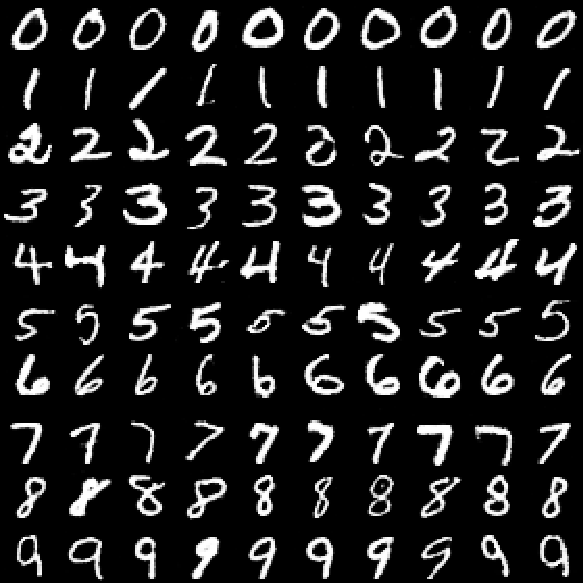
\includegraphics[width=0.3\textwidth]{figures/mnist/dcgan_mnist.pdf} & 
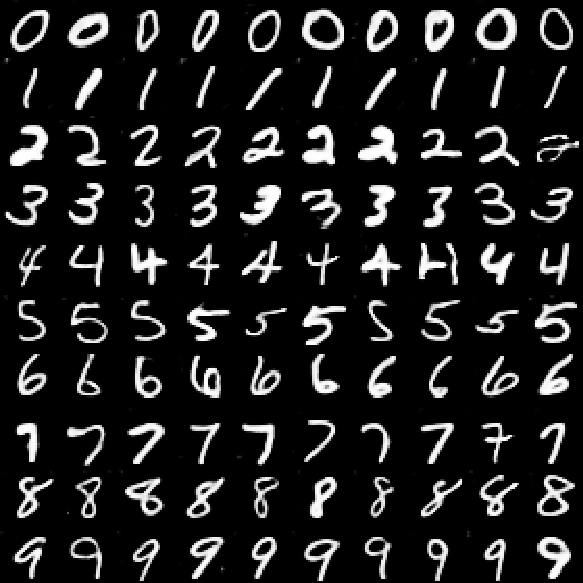
\includegraphics[width=0.3\textwidth]{figures/mnist/mnist_steingan.pdf}   \\
%\includegraphics[width=0.2\textwidth]{figures/mnist/vgd_gan_small.pdf} \\
DCGAN & SteinGAN \\
\vspace{5\baselineskip}
\end{tabular}
\begin{comment}
\renewcommand{\arraystretch}{1.2}
\begin{tabular}{|l|c|c|c|}
\hline
Training Data & Real Images & DCGAN %& SteinGAN (w/o kernel) 
& SteinGAN \\
\hline
Testing Accuracy& 92.58 \% &  41.82 \%  %& 62.93 \% 
& 58.69 \%\\
\hline
\end{tabular}
\end{comment}
\caption{
 MNIST images generated by DCGAN and our SteinGAN. We use the joint model in \eqref{equ:pxy} to allow us to generate images for each digit. We set $m = 0.2$. 
%Upper: MNIST images generated by DCGAN and our SteinGAN conditional on each digit. We use the joint model in \eqref{equ:pxy} to allow us generate images for each digit. Lower: Testing accuracy when using simulated images (of the same size as the real training set) to train ResNets for classification. SteinGAN achieves higher testing accuracy than DCGAN.
}
\label{fig:mnist}
\end{figure}



\begin{figure}[t]
\centering
\begin{tabular}{ccc}
\raisebox{8.3em}{
\renewcommand{\arraystretch}{1.5}
\newcommand{\tmpfnt}{\small}
\hspace{-.04\textwidth}
\begin{tabular}{r}
\tmpfnt airplane \\
\tmpfnt automobile \\
\tmpfnt bird \\
\tmpfnt cat \\
\tmpfnt deer \\
\tmpfnt dog \\
\tmpfnt frog \\
\tmpfnt horse \\
\tmpfnt ship \\
\tmpfnt truck
\end{tabular}} & 
\hspace{-.04\textwidth}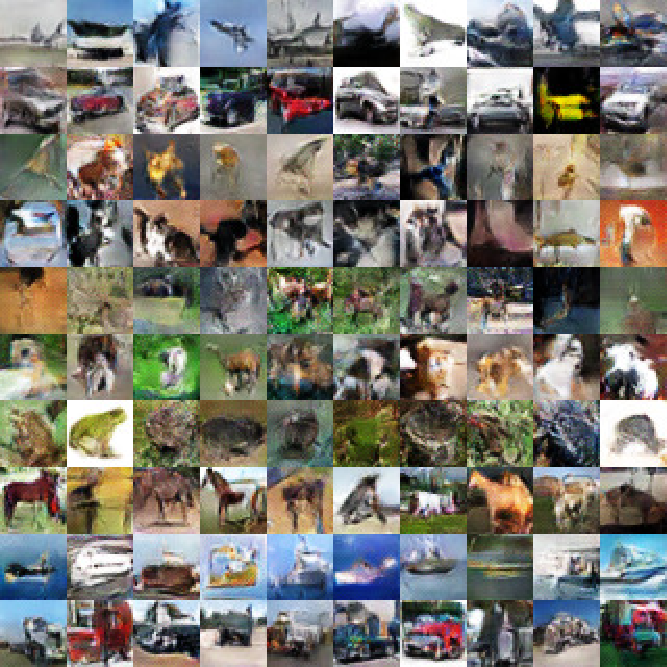
\includegraphics[width=.42\textwidth]{figures/cifar10/dcgan_cifar10.pdf}  & 
%\includegraphics[width=.3\textwidth]{figures/cifar10/vgd_no_kernel_cifar10.png}  & 
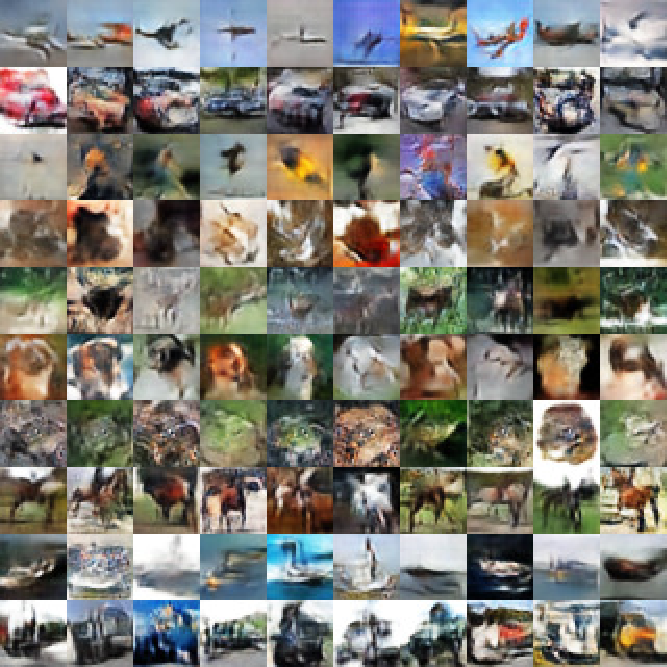
\includegraphics[width=.42\textwidth]{figures/cifar10/vgd_cifar10.pdf}  \\
& DCGAN 
%& SteinGAN (w/o kernel) 
& SteinGAN \\
\vspace{5\baselineskip}
\end{tabular}
\renewcommand{\arraystretch}{1.2}
\begin{tabular}{|l|c|c|c|c|}
\hline
\multicolumn{5}{|c|}{Inception Score} \\
\hline
 & Real Training Set & 500 Duplicate  & DCGAN  & SteinGAN \\
\hline
%Model Trained on ImageNet  & 11.237 & 11.100 & 6.581 & 6.209 \\
Model Trained on ImageNet  & 11.237 & 11.100 & 6.581 & 6.351 \\ %6.3514
\hline
%Model Trained on CIFAR-10 & 9.848 & 9.807 & 7.193 & 7.065 \\
Model Trained on CIFAR-10 & 9.848 & 9.807 & 7.368  & 7.428 \\  %7.368 % 7.193
\hline 
\end{tabular}  \\
\renewcommand{\arraystretch}{1.2}
\begin{tabular}{|c|c|c|c|}
\hline
\multicolumn{4}{|c|}{Testing Accuracy} \\
\hline
Real Training Set & 500 Duplicate  & DCGAN  & SteinGAN \\
\hline
92.58 \% &  44.96 \% & 44.78 \%  & 63.81 \%\\  %62.72 %63.81
\hline
\end{tabular}
\caption{Results on CIFAR-10. ``500 Duplicate'' denotes  500 images randomly subsampled from the training set, each duplicated 100 times.
Upper: images simulated by DCGAN and SteinGAN (based on joint model \eqref{equ:pxy}) conditional on each category.  
Middle: inception scores for samples generated by various methods (all with 50,000 images) on inception models trained on ImageNet and CIFAR-10, respectively. 
Lower: testing accuracy on real testing set when using 50,000 simulated images to train ResNets for classification. SteinGAN achieves higher testing accuracy than DCGAN. We set $m=1$ and $\gamma=0.8$.}%even though the images on in the upper panel look almost equally good visually.}
\label{fig:cifar10}
\end{figure}


\begin{figure}[t]
\centering
\begin{tabular}{cc}
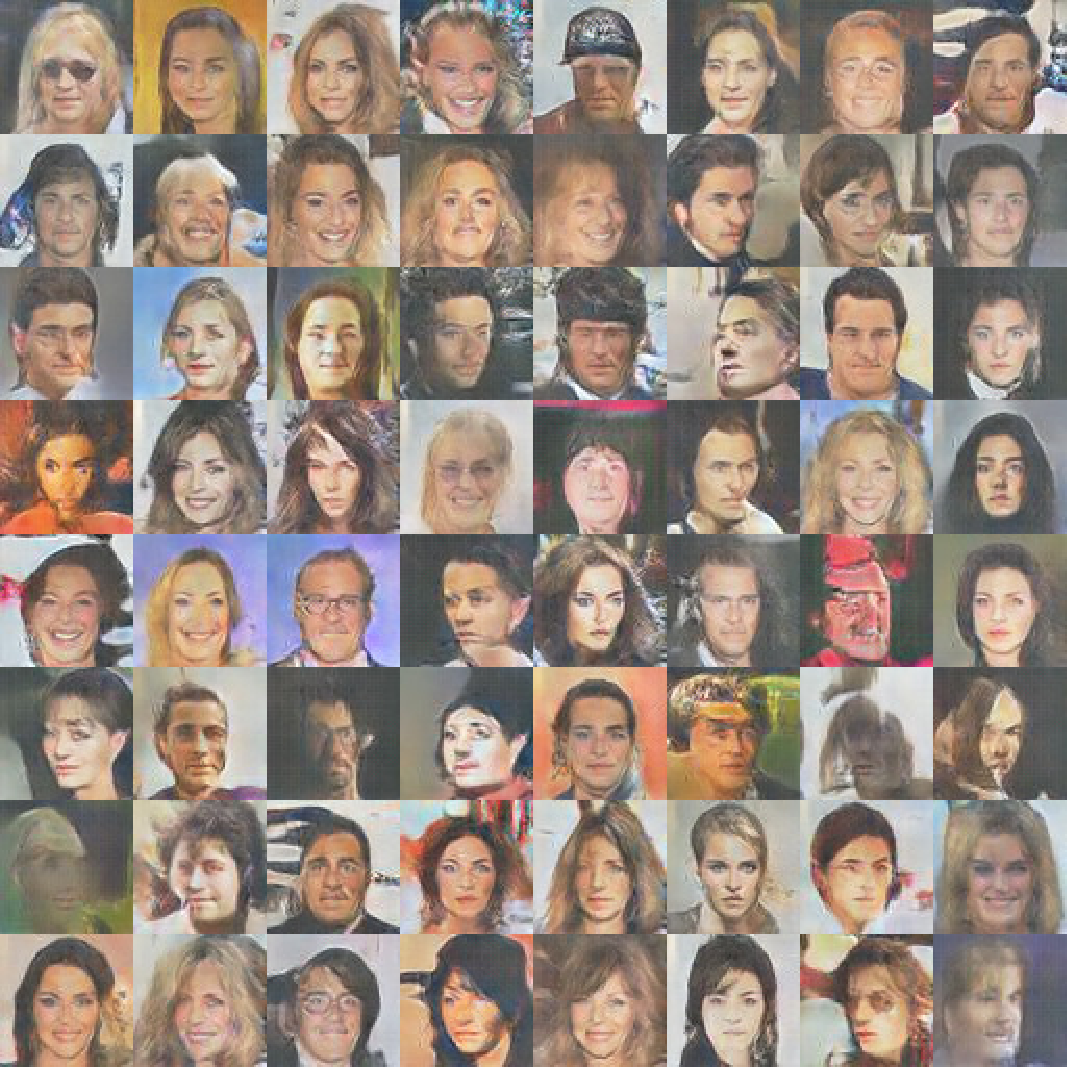
\includegraphics[width=0.45\textwidth]{figures/faces/dcgan_bright.pdf} & 
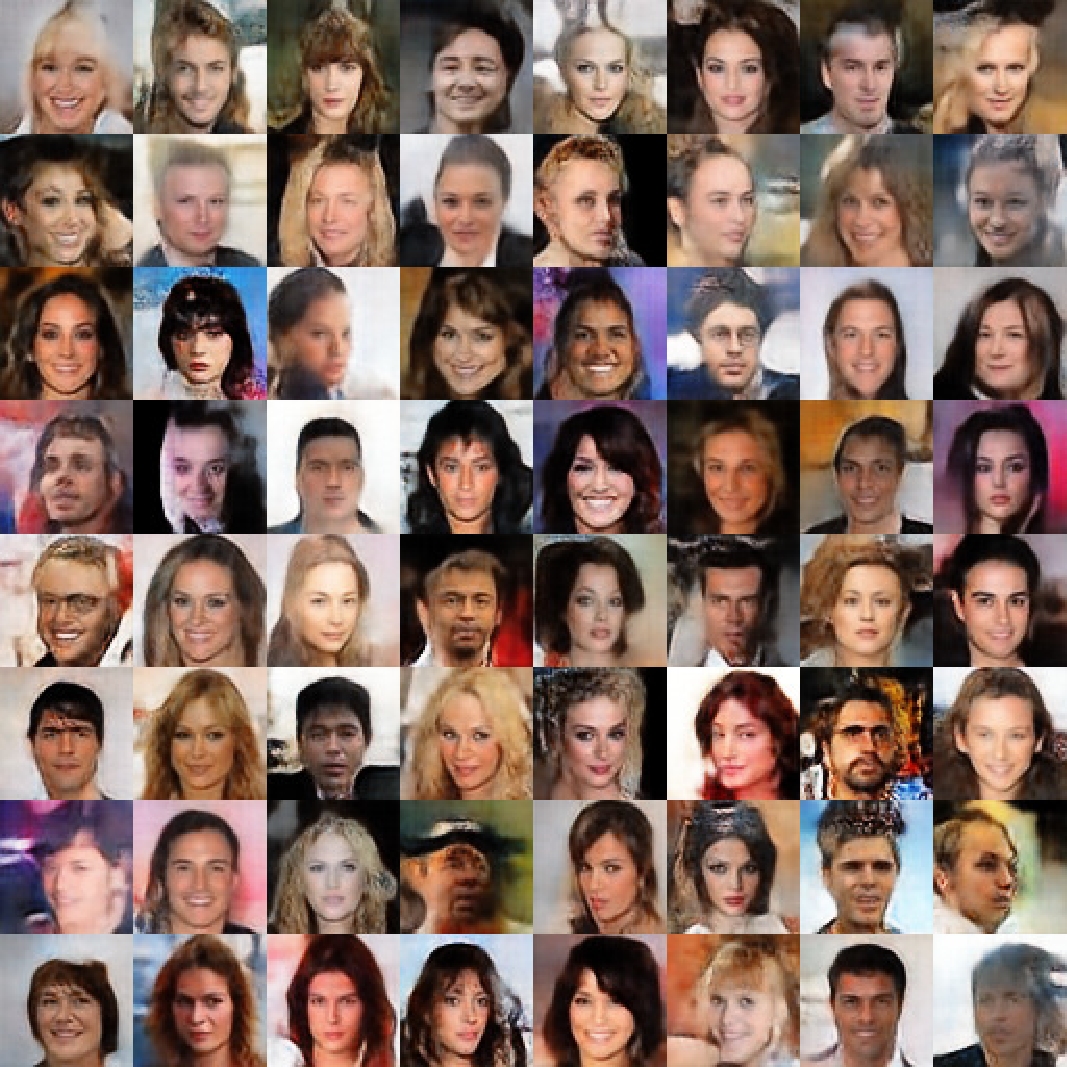
\includegraphics[width=0.45\textwidth]{figures/faces/vgd_faces_small.pdf} \\
DCGAN & SteinGAN \\
\end{tabular}
\begin{tabular}{c}
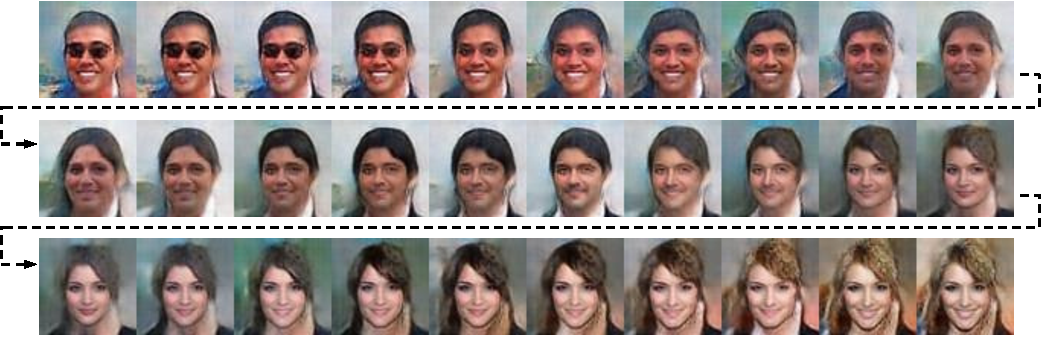
\includegraphics[width=0.85\textwidth]{figures/faces/z2.pdf} \\
\end{tabular}
\caption{Results on CelebA. Upper: images generated by DCGAN and our SteinGAN. Lower: images generated by SteinGAN when performing a random walk $\xi\gets \xi + 0.01\times\mathrm{Uniform}([-1,1])$ on the random input $\xi$; we can see that a man with glasses and black hair gradually changes to a woman with blonde hair. 
See Figure~\ref{fig:facemore} for more examples. }
%It can be observed that a generation of a man with glasses is gradually changed to a woman with blonde hair, all of which make a lot of sense.}
\label{fig:face}
\end{figure}


\begin{figure}[t]
\centering
\begin{tabular}{cc}
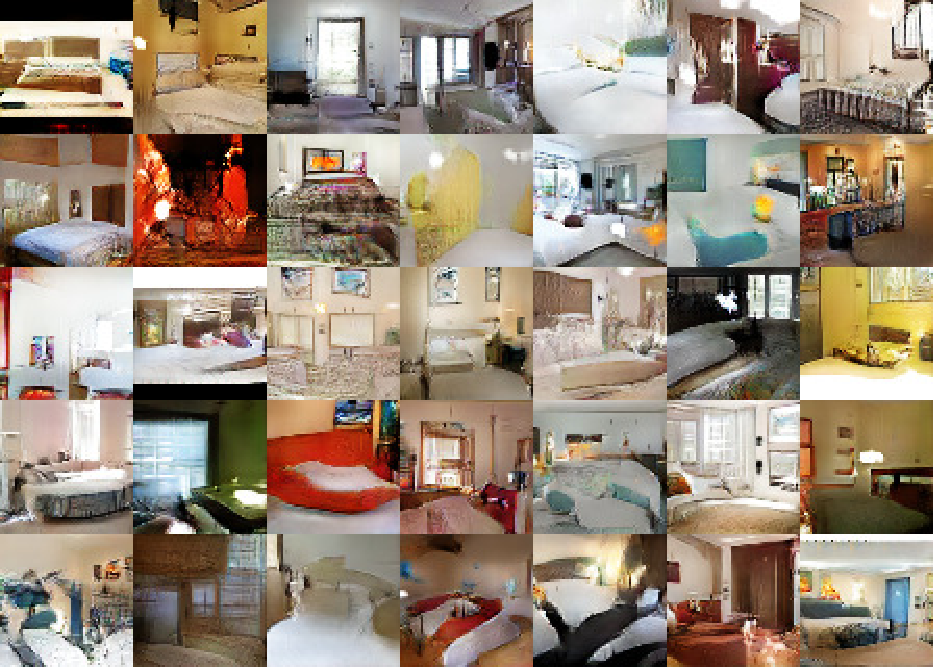
\includegraphics[width=0.45\textwidth]{figures/lsun/dcgan_5_7.pdf} & 
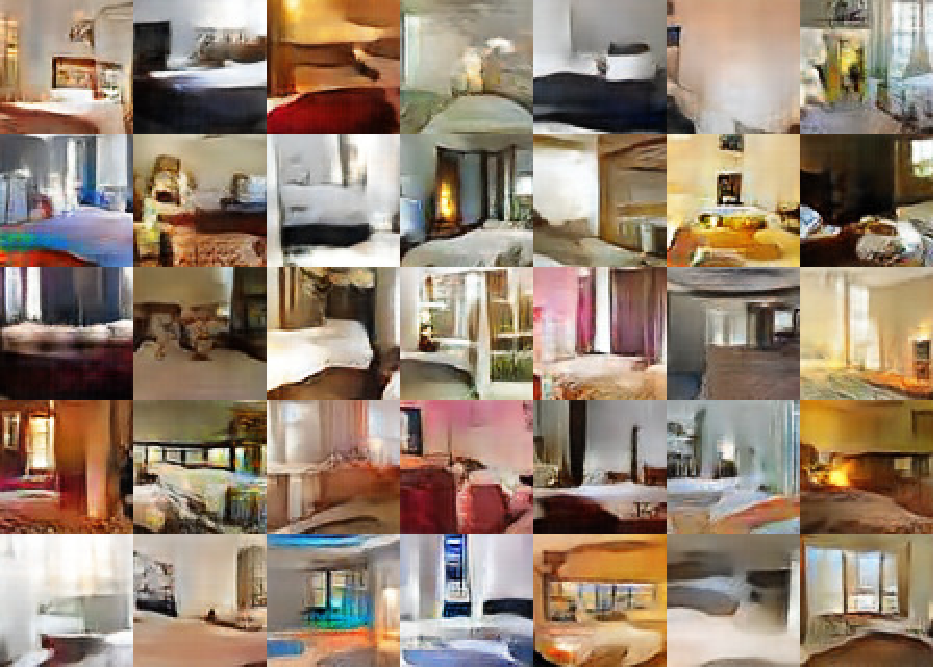
\includegraphics[width=0.45\textwidth]{figures/lsun/vgd_5_7.pdf} \\
DCGAN & SteinGAN\\
\end{tabular}
\caption{Images generated by DCGAN and our SteinGAN on LSUN.}
\label{fig:room}
\end{figure}


\begin{comment}
\begin{figure}[h]
\centering
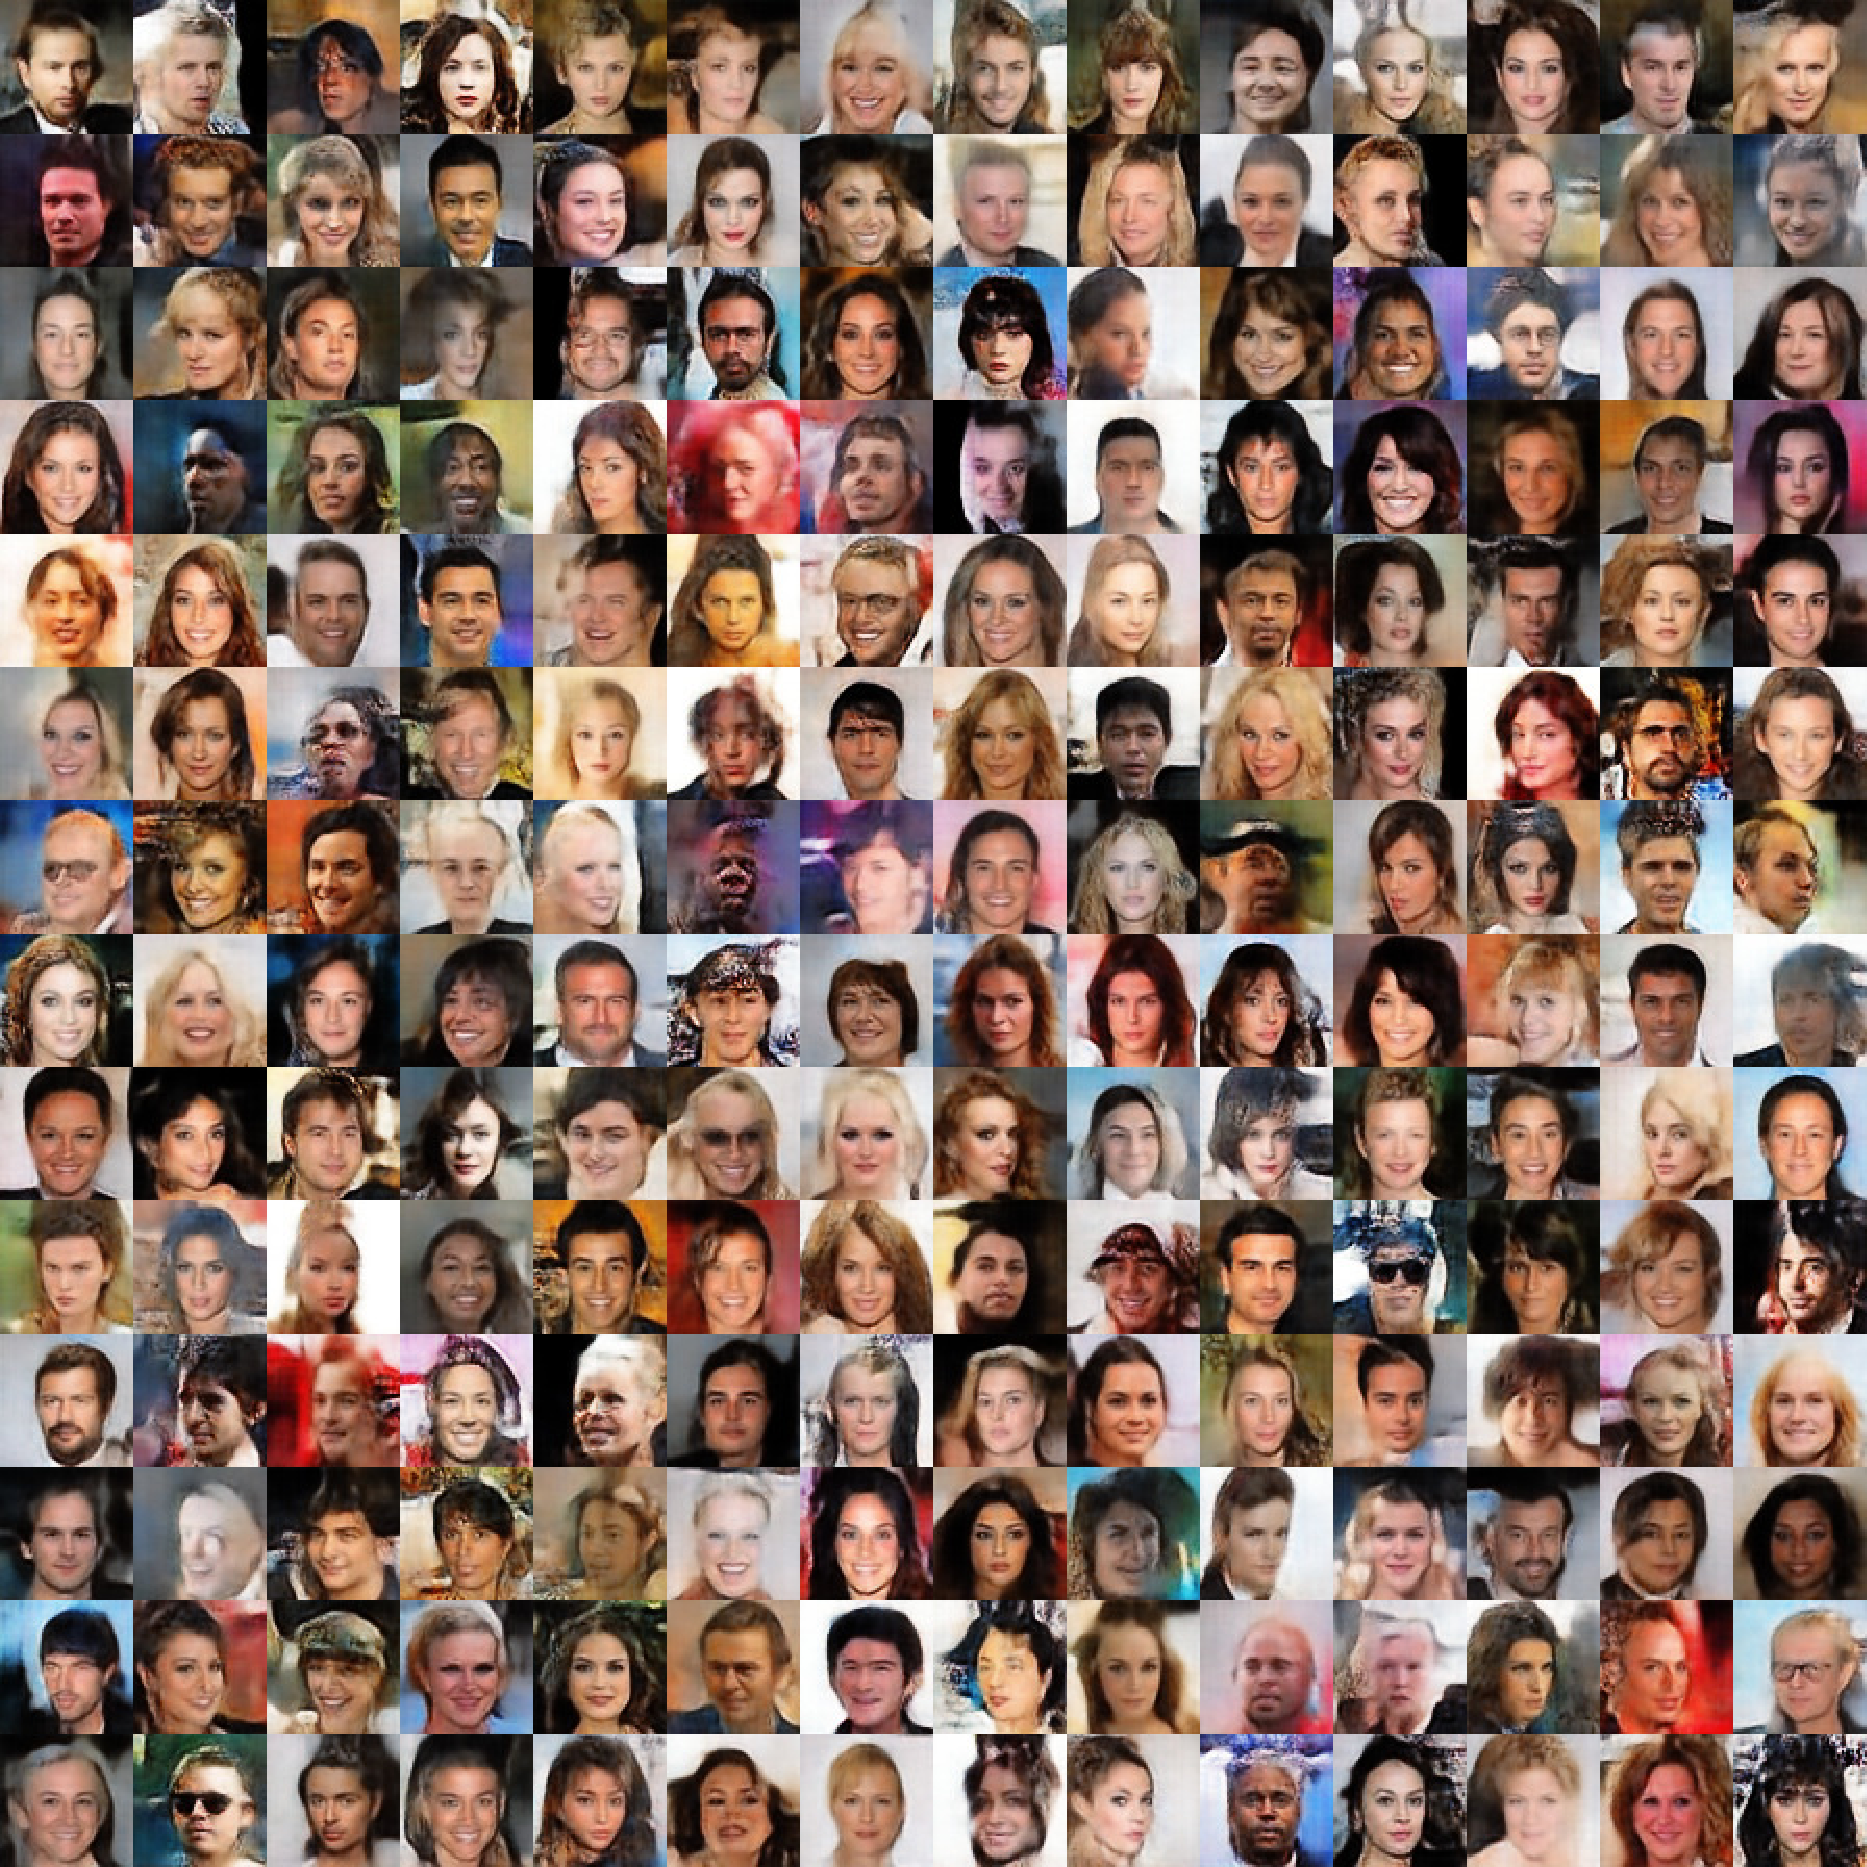
\includegraphics[width=0.9\textwidth]{figures/faces/vgd_gan-20.pdf}  
\caption{More images generated by SteinGAN on CelebA.}
\label{fig:facemore}
\end{figure}

\end{comment}
